% Prepared by Calvin Kent
%
% Assignment Template v19.02
%
%%% 20xx0x/MATHxxx/Crowdmark/Ax
%
\documentclass[12pt]{article} %
\usepackage{CKpreamble}
\usepackage{CKassignment}
\usepackage{tkz-euclide}
\usepackage{physunits}
\usepackage{physics}
\usepackage{lmodern}
\usepackage{microtype}
\usepackage{tasks}
\usepackage{upgreek}
\usepackage{xcolor}
\usepackage{euscript}
\usepackage{tasks}
\usepackage{tkz-euclide}
\usepackage{upgreek}
\usepackage[misc]{ifsym}


\usepackage{pgfplots}
\usepgfplotslibrary{polar}
\usepgflibrary{shapes.geometric}
\usetikzlibrary{calc}


\usepackage{euscript}
\usepackage{microtype}
\usepackage{upgreek}
\usepackage[misc]{ifsym}

%%Title
\title{Functions Test 2}
\date{January 17, 2021}

%%% Maths and science packages

\usepackage{amsmath,amsthm,amssymb}
\usepackage{pgfplots}
	\usetikzlibrary{
		calc,
		patterns,
		positioning
	}
	\pgfplotsset{
		compat=1.16,
		samples=200,
		clip=false,
		my axis style/.style={
			axis x line=middle,
			axis y line=middle,
			legend pos=outer north east,
			axis line style={
				->,
			},
			legend style={
				font=\footnotesize
			},
			label style={
				font=\footnotesize
			},
			tick label style={
				font=\footnotesize
			},
			xlabel style={
				at={
					(ticklabel* cs:1)
				},
				anchor=west,
				font=\footnotesize,
			},
			ylabel style={
				at={
					(ticklabel* cs:1)
				},
				anchor=west,
				font=\footnotesize,
			},
			xlabel= $x$,
			ylabel=$\vec d (\m \tx{[East]})$
		},
	}
	\tikzset{
		>=stealth
	}

\pgfplotsset{my style/.append style={axis x line=middle, axis y line=
middle, xlabel={$t$}, ylabel={$y[\text{m}]$}, axis equal }}


%%% Tables and figures packages

\usepackage{float}
\usepackage{caption}
	\captionsetup{
		format=plain,
		labelfont=bf,
		font=small,
		justification=centering
	}
	
%%% Numbers and sets

\newcommand{\E}{\mathrm{e}}

\newcommand{\tx}[1]{\text{#1}}

\begin{document}
    \pagenumbering{arabic}
    % Start of class settings ...
    \renewcommand*{\coursecode}{MCR3U Quiz} % Quiz Title
    \renewcommand*{\assgnnumber}{1} % Quiz number
    \renewcommand*{\submdate}{November, 2021} % renew the date
    \renewcommand*{\studentfname}{\textbf{Name:}} % Student first name
    \renewcommand*{\studentlname}{} % Student last name
    %\renewcommand*{\studentnum}{SNumber} % Student number

    \renewcommand\qedsymbol{$\blacksquare$}
    \setfigpath
    % End of class settings 
    \newgeometry{left=18mm, right=18mm, top=22mm, bottom=22mm} % page is set to default values
    \fancyhfoffset[L,O]{0pt} % header orientation fixed
    % End of class settings
    %%% Note to user:
    % CTRL + F <CHANGE ME:> (without the angular brackets) in CKpreamble to specify graphics paths accordingly.
    % The command \circled[]{} accepts one optional and one mandatory argument.
    % Optional argument is for the size of the circle and mandatory argument is for its contents.
    % \circled{A} produces circled A, with size drawn for letter A. \circled[TT]{A} produces circled A with size drawn for TT.
    % https://github.com/CalvinKent/My-LaTeX
    %%%
    % Crowdmark assignment start


    %%%%%%%%%%%%%%%%%%%%%%%%%%%%%%%%%%%%%%%%%%%%%%%%%%%%%%%%%%%%%%%%%%%%%%%%%%%%%%%%%%%%%%%%%%%%%%%%%%%%%%%%
    %%%%%%%%%%%%%%%%%                  PROBLEM IDEAS                  %%%%%%%%%%%%%%%%%%%%%%%%%%%%%%%%%%%%%%
    %%%%%                   ----------------------------------------                                %%%%%%%%

    % --> Do a hard tangent line problem

	\maketitle
	\section{Preamble}
	This is a test covering what we have learnt so far in lecture. Student's \emph{\textbf{must show all work}} to receive full marks.
	\section{Allowed Aids}
	The following aids are allowed on the Test
	\begin{itemize}
    \item \textbf{Open Book Test} (Your entire binder is allowed).
	\end{itemize}
	\section{Restrictions:}
  \begin{itemize}
		\item \textbf{NO} calculator's.
  \end{itemize}
  \section{Remarks:}
  \begin{itemize}
    \item $n\cdot \textbf{S} = \underbrace{\textbf{S} + \dots + \textbf{S}}_{\text{n times}}$. \hfill $(n \in
      \mathbb N)$
    \item $\operatorname{len}(\textbf{S})$ is number of bits in the binary string $\textbf{S}$.
    \item $\operatorname{floor}(x)$ is the smallest integer less than or equal to $x$.
  \end{itemize}
	\section{Name and Date:}
	Print your name and todays date below;

  \vspace*{0.4cm}

	\begin{center}
	\noindent\begin{tabular}{ll}
		\makebox[3in]{\hrulefill} & \makebox[3in]{\hrulefill}\\
		Name & Date\\[8ex]% adds space between the two sets of signatures
	\end{tabular}
	\end{center}
	\newpage


\section*{Part A - Multiple Choice}
\begin{qstn} % qnumber, qname, qpoints
  Answer the following True/False questions,
  \begin{enumerate}
    \item Let $\operatorname{id}_\R \colon \R \to \R$ be the identity function on $\R$, then
       \[
              \operatorname{id}_\R\left(\operatorname{id}^{-1}_\R\left(\operatorname{id}_\R\left(\operatorname{id}^{-1}_\R\left(\operatorname{id}_\R\left(\operatorname{id}^{-1}_\R\left(-4
              \right) \right) \right) \right) \right) \right) = 4
      .\] 
      Circle the correct answer: \,\, \textbf{True} \,\,\,\,\,\, \textbf{False}

    \item Let $f \colon \R \to \R$, $f(x) = 2(x - 1)^2$ be a function. Then $f$ is not invertible. \\
      \textbf{Hint: }Try using the Horizontal line test.\\
      Circle the correct answer: \,\, \textbf{True} \,\,\,\,\,\, \textbf{False}

    \item Let $ \mathcal{X} = \{0.5, \pi, 3.8\} $ and $ \mathcal{Y} = \{1,4,4.8\} $ be sets, define the
            following function, 
            \begin{itemize}
              \item $\mathcal{\psi} \colon \mathcal{X} \to \mathcal{Y}$.
              \item $\mathcal{\psi}(x) = \operatorname{floor}(x) + 1$.
            \end{itemize}
            Then $\psi$ is an invertible function.\\
          Circle the correct answer: \,\, \textbf{True} \,\,\,\,\,\, \textbf{False}
   \item Let $ \EuScript{S} = \{10,1100, 111000\} $ be a set of $\textit{binary strings}$ and $ Y =
     \{5,7,3\} $ be a set of natural numbers, define the following function, 
              \begin{itemize}
                \item $\Delta \colon \EuScript{S} \to Y$.
                \item $\Delta(\textbf{S}) = \operatorname{len}(\textbf{S}) + 1$.
              \end{itemize}
              Then the function,
              \begin{itemize}
                \item $\Delta^{-1} \colon Y \to \EuScript{S}$.
                \item $\Delta^{-1}(y) = \operatorname{floor}(y / 2)\cdot \textbf{1} + \operatorname{floor}(y /
                  2)\cdot \textbf{0}$,
                  \,\,\,\,(where $\textbf{1}$ and $\textbf{0}$ are $\textit{binary strings}$),
              \end{itemize}
              is the inverse function for $\Delta$.\\
      Circle the correct answer: \,\, \textbf{True} \,\,\,\,\,\, \textbf{False}

    \item Let $g(x) = \sqrt{x - 4} - 1$ be a function, then $g^{-1}(x) = (x-1)^2 + 4 $ is the inverse of
      $g$.\\
      Circle the correct answer: \,\, \textbf{True} \,\,\,\,\,\, \textbf{False}

    \item Let $f(x) = x^2 $. Suppose we apply the following transformations to $f$,
      \begin{itemize}
        \item Reflection across the y-axis.
        \item Vertical compression by a factor of $3$. 
        \item Horizontal compression by a factor of $2$.
        \item Horizontal shift, left by $2$ units.
        \item Vertical shift, down by $2$ units.
      \end{itemize}
      Then the corresponding transformation equation is $h(x) = \frac{1}{3}f(-2x - 4) - 2$.\\
      Circle the correct answer: \,\, \textbf{True} \,\,\,\,\,\, \textbf{False}

    \newpage

    \item Let $f(x) = \left|x\right|$, and let $h(x) = -2f(5x - 3) + 9$ be a transformation of $f(x)$, then the
      corresponding coordinate transformation of $f$ is,
       \[
           \left( x,f(x) \right)  \longrightarrow \left( \frac{x - 3}{5}, -2f(x) + 9 \right) 
      .\] 
      Circle the correct answer: \,\, \textbf{True} \,\,\,\,\,\, \textbf{False}

    \item Let $\Omega \colon \mathcal{H} \to \mathcal{T}$ be a $\textit{surjective function}$, then $
      \left|\mathcal{H}\right| = \left|\mathcal{T}\right|$.\\
      Circle the correct answer: \,\, \textbf{True} \,\,\,\,\,\, \textbf{False}

    \item Let $f(x) = x^2$ , let $h(x) = -f(x)$ be a transformation of $f$, and let $r(x) = -h(-x)$ be a
      transformation of $h$, then  $r(x) = f(x)$.\\
      Circle the correct answer: \,\, \textbf{True} \,\,\,\,\,\, \textbf{False}

    \item Let $f \colon \mathbb N \to \R$, $f(x) = x^2$ be a function. Then $f$ is not invertible. \\
      Circle the correct answer: \,\, \textbf{True} \,\,\,\,\,\, \textbf{False}



  \end{enumerate}
\end{qstn}

\newpage

\section*{Part B - Solve all problems}

\begin{qstn}
  For each of the following, you are given a function and its definition. For each question,
  \begin{enumerate}[label=(\alph*)]
    \item[(i)] Prove that the function is invertible \textbf{or} prove that the function is not invertible.
    \item[(ii)] Determine the range of the function.
  \end{enumerate}

  \begin{enumerate}[label=(\alph*)]
  \item Let $\EuScript{S} = \{1100,0011,1010\} $, $\EuScript{T} = \{0011,1010,0100,1100\}$ be sets of binary
    strings and define,
    \begin{itemize}
      \item $\lambda \colon \EuScript{S} \to \EuScript{T}$.
      \item $\lambda(\textbf{S}) = \vb s_3\vb s_4\vb s_1 \vb s_2$.
  \end{itemize}


    \vspace*{7cm}



  \item Let $\mathcal{N} = \{2.7,0.2,1.3,2.4\} $, $\mathcal{M} = \{0,2,4\}$ be sets and define,
    \begin{itemize}
      \item $\omega \colon \mathcal{N} \to \mathcal{M}$.
      \item $\omega(n) = 2\cdot \operatorname{floor}(n)$.
    \end{itemize}
  \end{enumerate}

\end{qstn}

\newpage

\begin{qstn}
  Let $\beta \colon V \to W$ be an invertible function. Suppose that the formula for the invertible function is,
  \[
      \beta^{-1}(w) = 2w - 4
  .\] 
  \begin{enumerate}[label=(\alph*)]
    \item Given the co-domain $W = \{-2,-4,0,2\} $ of $\beta$, recover the domain $V$.

    \vspace*{6cm}

  \item Determine the formula for $\beta(v)$.\\
    \textbf{Hint: }Use the same algorithm for determining the inverse.

    \vspace*{4cm}

  \item Confirm that your formula for $\beta(v)$ is correct by checking that each element in $V$ correctly maps back to the corresponding
        elements in $W$.

  \end{enumerate}
\end{qstn}

\newpage

\begin{qstn}
Let $ X = \{-3,0,-5\} $ and $ Y = \{5,3,0\} $ be sets, define the following function, 
\begin{itemize}
    \item $\Phi \colon X \to Y$.
    \item $\Phi(x) = \left|x\right|$.
\end{itemize}

Prove that the function,
\begin{itemize}
    \item $\Phi^{-1} \colon Y \to X$.
    \item $\Phi^{-1}(y) = -\operatorname{id}_Y(y)$.
\end{itemize}
is the inverse function for $\Phi$.

\end{qstn}


\newpage


\begin{qstn}
  Determine the inverse function for the following functions,
  \begin{enumerate}[label=(\alph*)]
    \item $f(x) = 4x + 8$.
        \vspace*{8cm}

    \item $H(x) = \sqrt{x - 16} + 2$.
  \end{enumerate}
\end{qstn}

\newpage

\begin{qstn}
Suppose that I throw a ball from ground level and my sister simultaneously throws a rock. She manages to hit the
ball at exactly $t=  3$ seconds.
      \begin{center}
      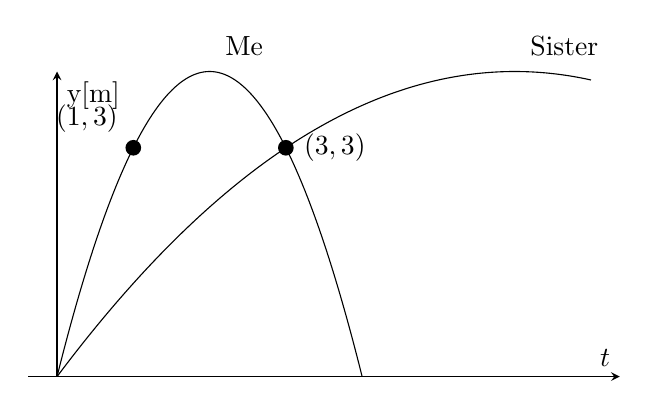
\begin{tikzpicture}
        \begin{axis}[
          my style,
          ytick=\empty,
          xtick=\empty,
          xticklabels=\empty,
          width=0.75\textwidth,
          height=0.45\textwidth,
          yticklabels=\empty,
          ylabel={y[m]}]

          \addplot[domain=0:4]{-(x -  2)^2 + 4};
          \addplot[domain=0:7]{-(0.3333333*x -  2)^2 + 4};

          \node[label={45:{\textcolor{black}{Me}}},circle,inner sep=2pt] at (axis cs:2,4) {};
          \node[label={45:{\textcolor{black}{Sister}}},circle,inner sep=2pt] at (axis cs:6,4) {};
          \node[label={0:{\textcolor{black}{$(3,3)$}}},circle,fill,inner sep=2pt] at (axis cs:3,3) {};

          \node[label={135:{\textcolor{black}{$(1,3)$}}},circle,fill,inner sep=2pt] at (axis cs:1,3) {};

        \end{axis}
      \end{tikzpicture}
      \end{center}
\end{qstn}
Let $M(x)$ denote my graph and $S(x)$ denote the graph of my sister. We can represent the graph of my sister as
a horizontal scaling of my graph, 
\begin{align*}
  S(x) = M(B\cdot x) \tag{$B \in \R, B \neq 1$}
\end{align*}
 Using the data given in the plot, determine the correct value for $B$.




\newpage

\begin{qstn}
  Let $f(x) = \left|x\right|$, and let $R(x) = -\frac{1}{2}f(2x + 4) + 1$ be a transformation of $f$. 
  \begin{enumerate}[label=(\alph*)]
    \item Describe the transformation.
        \vspace*{7cm}

    \item Determine the expression for the coordinate transformation,
      \[
          \left( \frac{x- H}{B}, Af(x) + K \right) =
          \left( \textcolor{white}{\frac{\text{  }}{\text{  }}} \hspace*{2.5cm}, 
            \textcolor{white}{\frac{\text{  }}{\text{ }}} \hspace*{2.5cm}\right) 
      \] 
      \vspace*{1cm}

    \item Complete the following coordinate table to determine the corresponding transformed coordinates.
        \begin{center}
          \begin{tabular}{c|c}
        \text{$\left( x,f(x) \right) $} & \text{$ \left( \textcolor{white}{\frac{\text{  }}{\text{  }}} \hspace*{2.5cm}, 
            \textcolor{white}{\frac{\text{  }}{\text{ }}} \hspace*{2.5cm}\right) $}\\\hline 
              \\
              $(0,0)$ & $\hspace*{9cm}$\\
              \\
              \\
              $(-6,6)$ & $\hspace*{9cm}$\\
              \\
              \\
              $(6,6)$ & $\hspace*{9cm}$\\
              \\
              \\
              $(-4,4)$ & $\hspace*{9cm}$\\
              \\
              \\
              $(4,4)$ & $\hspace*{9cm}$\\
              \\
              \\
        \end{tabular}

        \end{center}

  \newpage

   \item Using your results from the coordinate table, sketch the transformation $R(x)$. Be sure to
     \textbf{label} the transformed coordinates as well as the function.

    \begin{center}
        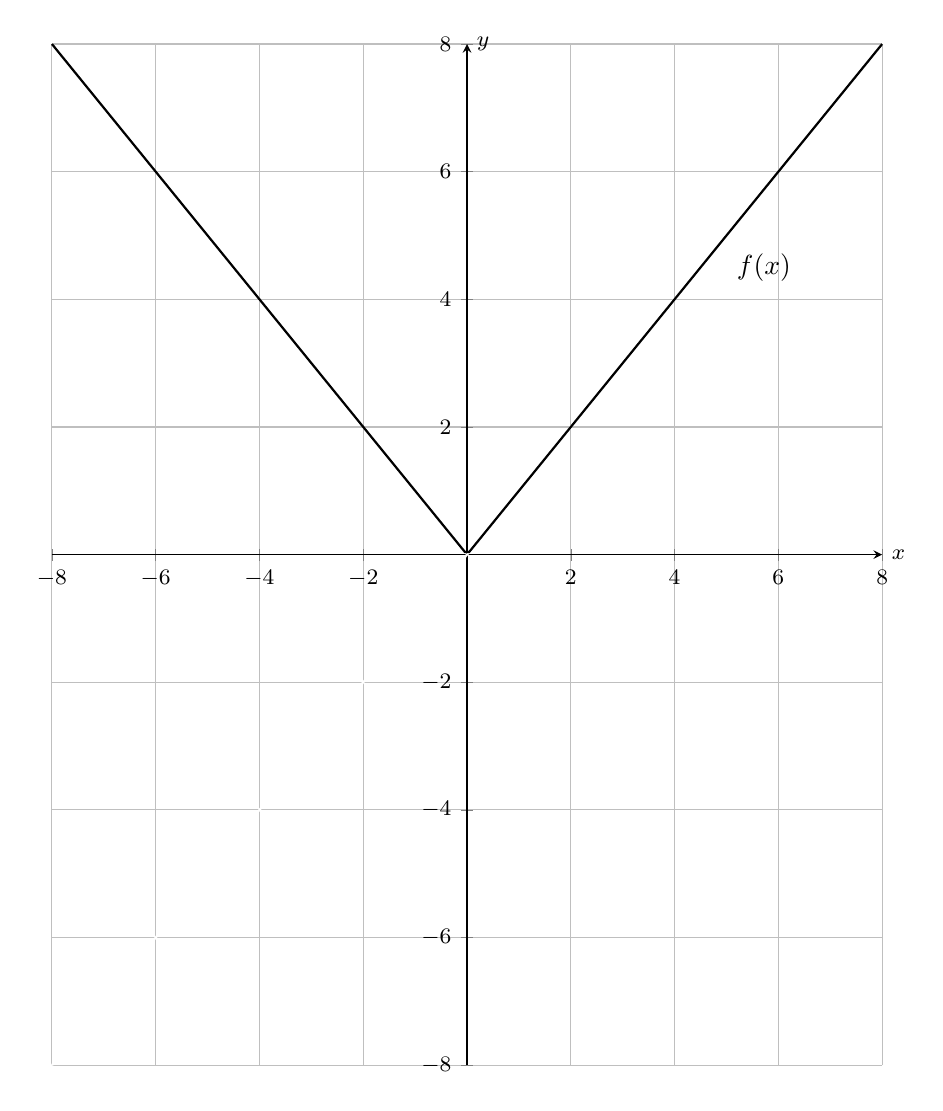
\begin{tikzpicture}
        \begin{axis}[
            my axis style,
            width=1\textwidth,
            height=1.2\textwidth,
            ylabel=$y$,
            grid
        ]
        
        \addplot[
            domain=-8:8,
            thick,
            white,
            -
        ]
        {x};
 
        \addplot[
            domain=-8:8,
            thick,
            black,
            -
        ]
        {abs(x)};

        \fill[
            black
        ];

        \node[label={275:{\textcolor{black}{$f(x)$}}},circle,inner sep=2pt] at (axis cs:5,5) {};

        \end{axis}
        \end{tikzpicture}
    \end{center}
  \end{enumerate}
\end{qstn}

\newpage


\section*{Part C - Solve exactly one of the three problems.} 

\begin{qstn}
  Let $A = \{a,b,c\}$, $B = \{x,y,z\}$ be sets. Let $\mathcal{L}$ be the set of all functions from $A \to B$. Let
  $\mathcal{M} = \{f \in \mathcal{L} \mid f \text{ is invertible}\} $. Determine $\left|\mathcal{M}\right|$ and
  justify that your answer is correct.\\
  \textbf{Note: }Try counting all possible mapping diagrams between $A$ and $B$. Two invertible functions are the same if their mapping diagrams are equivalent.
\end{qstn}

\begin{qstn}
  Let $A,B$ be sets, and let  $F \colon A \to B$ be a function between the sets. We define the \textbf{nullset} of
  $F$ to be,
  \[
        \text{Null}(F) = \{a \in A \mid F(a) = 0\} 
  .\] 
  Let $G \colon \R \to \R$, $G(x) = 2x - 4$,
   \begin{enumerate}[label=(\alph*)]
     \item Determine $\text{Null}(G)$.
     \item What do you think $\text{Null}(G^{-1})$ contains and why?
     \item Determine $\text{Null}(G^{-1})$.
  \end{enumerate}
  
\end{qstn}

\begin{qstn}
  Consider the following grid below,
  \begin{center}
    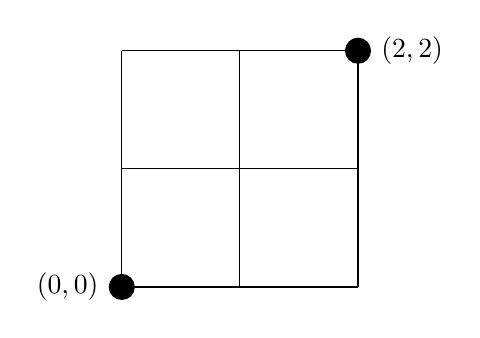
\begin{tikzpicture}
    \draw[step=1.5cm,color=black] (0,0) grid (3,3);

        \node[label={0:{\textcolor{black}{$(2,2)$}}},circle,fill] at (3,3) {};
        \node[label={180:{\textcolor{black}{$(0,0)$}}},circle,fill] at (0,0) {};

    \end{tikzpicture}
  \end{center}

  Let \texttt{R} denote a rightward move and \texttt{U} denote an upward move. We define a path from $(0,0)$ to  $(2,2)$ to be a 
  sequence of rightward and upward moves. For example \texttt{RRUU} is a path from $(0,0)$ to  $(2,2)$, and so is
  \texttt{UURR}.

  \begin{enumerate}[label=(\alph*)]
    \item Determine all paths from $(0,0)$ to  $(2,2)$. Collect all of these paths into the set $\EuScript{P}$.\\
      \textbf{Hint:} $\left|\EuScript{P}\right| = 6$.
    \item Let $Z = \left\{ \{1,2\}, \{1,3\}, \{1,4\}, \{2,3\}, \{2,4\} , \{3,4\}\right\} $.
      \begin{enumerate}[label=(\alph*)]
        \item [(i)]Describe a function $\Psi \colon \EuScript{P} \to Z$ that assigns a 
          relationship between the two sets.\\
          \textbf{Note:} The function description can be in words.
        \item [(ii)] Draw a mapping diagram for $\Psi$ based on your description of the function.\\
          \textbf{Hint:} In my description : $\Psi(\texttt{UURR}) = \{3,4\}, \Psi(\texttt{RUUR}) = \{1,4\} $
          (Yours could be different)\\

      \end{enumerate}
  \item Describe the inverse function $\Psi^{-1} \colon Z \to \EuScript{P}$.\\

  \end{enumerate}

  \textbf{\large{CHOOSE AND SOLVE ON NEXT PAGE}}
  
\end{qstn}

\newpage

\textbf{Question} \underline{\hspace*{1cm}}.



\end{document}






























